\chapter{Three Dimensional Visualization and Web Development}

As any software project, this visualization tool also relies on many different algorithms and technical standards or conventions. This chapter aims to give an overview of the major external components and ideas, that contribute to the project and the way it works.
\section{Algorithms}
\subsection{Marching Cubes Algorithm} \label{chp2:Cubes}
The marching cubes algorithm was designed in 1987 and published in \cite{MarchCubes}. The original idea was to create high resolution triangle models of constant density surfaces for medical purposes. However, the algorithm can be applied to any three dimensional scalar data set, not only tissue density. The aim of the algorithm is to find an isosurface within a data set. An isosurface is a two dimensional surface within a three dimensional context, that connects the points in space in which the data set has the same value.\footnote{Compare contour lines on a two dimensional map.}

The algorithm uses the ``divide and conquer'' approach. It divides the whole set into small cubes, which it then iterates or `marches' through. The cubes are evaluated at the corners and each one gets marked, if it exceeds the isosurface value $val_{iso}$. That leads to $2^8=256$ different ways for a cube to be marked. Based on the marked corners, triangles are inserted within the cube, so they separate the marked corners from the unmarked ones. This is a clever way, because if a corner with a higher value is adjacent to one with a lower value, the isosurface has to intersect the edge somewhere in between. In order to further enhance the accuracy of the surface, a linear interpolation is used, to decide where on each edge of the cube the corners of the triangle(s) should be placed. Using two different symmetries the actual number of triangle arrangements can be reduced to 14. In each of those there is up to four triangles, as can be seen in figure \ref{fig:cubes-arr}.
\begin{figure}\begin{center}
  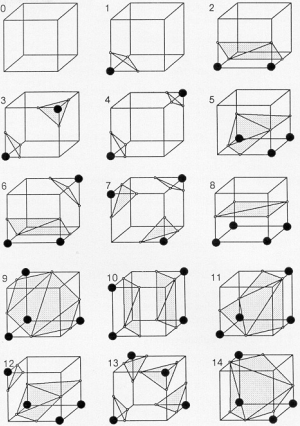
\includegraphics[width=0.45\textwidth]{pictures/cubes_arrangements}
  \caption[Tringles arrangements]{Tringles arrangements. as seen in \cite{MarchCubes}}\label{fig:cubes-arr}
\end{center}\end{figure}

Most implementations of the Marching Cubes Algorithm use lookup tables to store which edges get intersected, based on the marked corners. This makes sense, since an array lookup is a very cheap instruction, when it comes to processing time and an array with 256 entries usually is not too big. Especially in comparison to the number of triangles that is needed for a satisfying reconstruction of any realistic 3D-surface.

\section{File Types}
\subsection{Shapefile}
A shapefile stores attribute and geometry information. Geometries are represented by shapes consisting of a set of vector coordinates. As it can be seen in its technical description~\cite{ersi:shp} a shapefile actually consists of more than one file. There are at least three parts to every shapefile. A main file, an index file and a dBASE table. The files are all named by the same valid filename. The suffix however distinguishes between the main (.shp), the index (.shx) and the dBase (.dbf) files.

The main file grants direct access to the geometrical information. It consists of a \unit[100]{byte} header followed by variable-length records. The header contains file management information, like the file code, file length, etc. It also gives information on the data set, like bounding box coordinates and shape type. The records represent the actual shapes. Each record consists of an \unit[8]{byte} record header and a variable sized list of vertices. The record header simply contains the record number and its length. The length depends on what shape is represented and how many vertices it is made up of. The organization of the main file can be seen in figure~\ref{fig:main-orga}.
\begin{figure}\begin{center}
  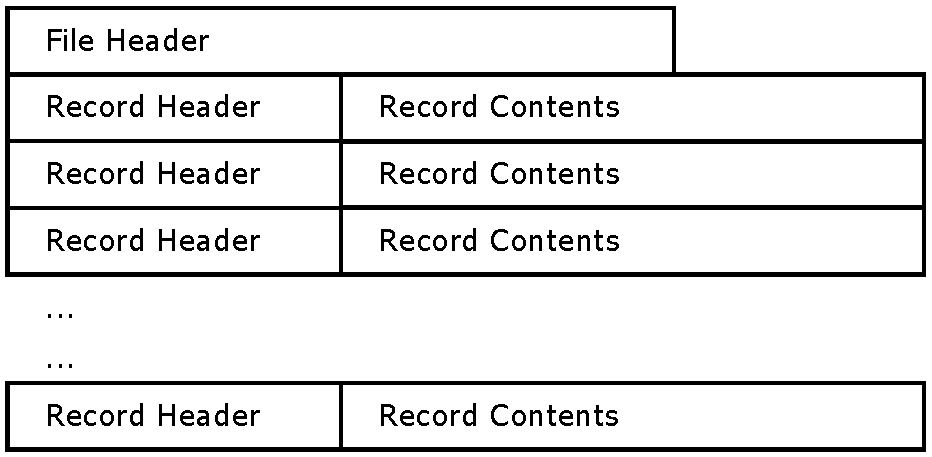
\includegraphics[width=0.8\textwidth]{pictures/Shapefile}
  \caption[Organization of the Main File]{Organization of the Main File. as seen in \cite{ersi:shp}}\label{fig:main-orga}
\end{center}\end{figure}

The index file also starts with a \unit[100]{byte} header, which is identical to the main file header. After that, there is a record entry for each of the records in the main file. The $i^{th}$ record entry contains the length of the $i^{th}$ record in the main file and its offset relatively to the beginning of the file.

The dBASE file contains additional attributes concerning the shapes. The format is a standard DBF file, that is used by many applications with only a few extra requirements. The record order for example has to be the same as the order of the shapes in the main file.

\subsection{ODA files}
The ODA file format is a simple way to to store geometrical information about urban outdoor environments. This format is especially interesting, because it is used by the WallMan~\cite{WallMan} application in the WinProp wireless network planning software package~\cite{WinProp}. It is a simple ASCII format.

The file starts with a header of six lines, consisting of five lines of comment and one line of general database settings. The body of the file consists of two blocks. The first block contains some material information, which is  referred to in the second block. That block holds the actual outdoor building data. All buildings are represented by an arbitrary number of 2D-coordinates, outlining the base shape, and one height parameter.

\subsection{APA file}
The APA file format is an ASCII based format used by the AMan~\cite{AMan} application, which is also part of the WinProp wireless network planing software package~\cite{WinProp}. It stores three dimensional antenna gain patterns. APA files mostly consist of data triples. There can only be one triple per line and it must be made up of two angular values (horizontal and vertical) and one gain value (in \unit{dB}).

\subsection{CSV file}
The CSV~\cite{CSV} file format is a widely used, ASCII based, format. It is able to represent any kind of tabular data. Different characters can be used to separate the data values. The line break character usually signifies the end of a data record. Within each record there can be multiple data fields, separated by a special character\footnote{The comma is usually used for that, but semicolon, colon, tab or space are alternatives.}.

\section{Rendering and Output}
\subsection{Rendering Basics}
\subsection{Three.js WebGL Framework}
Three.js is a JavaScript based API\@. It uses WebGL~\cite{WebGL}. Therefore it provides the opportunity to use hardware accelerated 3D-graphics inside of HTML5 browsers, making it platform independent.

The framework was first published in 2010 by Ricardo Cabello, also called {``mrdoob''} online.~\cite{ThreeWhite} He started with 3D modeling and editing together with other programmers. When he felt, that the tools he used to create his animation scenes were not satisfying his needs, he started do develop his own framework. When finally JavaScript and WebGL support started to get better, he ported this project from ActionScript to JavaScript an published it on GitHub\footnote{available on: https://www.github.com/mrdoob/three.js}. Since then many contributors are still taking part in the development of that project.

The aim of the framework is to abstract the work and theoretical calculations, that come up when a three dimensional scene is rendered to a two dimensional screen. It provides developers with classes and methods that are convenient for the fast and easy creation of three dimensional scenes. Implemented are many usefull features~\cite{ThreeFeatures} like:
\begin{description}
\item[Different Renderes] are available, including WebGl, Canvas and SVG renderer
\item[Scenes] can be edited at run-time
\item[Cameras and Controllers] in many different varieties.
\item[Lighting] can be added to a scene like any object; Shadows are calculated internally
\item[Materials] with different shadow and texture options are provided.
\item[Geometries] both custom made and predefined (cube, sphere, torus, \ldots)
\item[Loaders] for images, JSON objects and more
\item[Examples] are provided on nearly every functionality the framework provides
\end{description}
All this lets the developers working with three.js focus more on designing an creating the scene, rather than on the difficulties of displaying it on the computer screen. However, should a special case arise and the developer needs to work on a more basic level, that is no problem. Three.js can incorporate any self-written shaders and posses a variety of utility math functions, like matrix and vector calculation and projection.

Listing~\ref{list:example} shows an easy example on how to use three.js in a JavaScript document. The code creates a Scene, a PerspectiveCamera, and a WebGLRenderer object. The renderer is then added to the body of the HTML page. Afterwards the predefined BoxGeometry and MeshBasicMaterial classes are used to create the mesh of a simple 1x1x1 cube. Finally, it is added to the scene and the camera is moved. Now the rendering loop is started, which slowly rotates the cube around the x and y axis. This example shows how a relatively complex animation can easily be implemented with just a few lines of code.
\lstset{
caption=Three.js Example,
label=list:example,
language=JavaScript}
\begin{lstlisting}
var scene = new THREE.Scene();
var camera = new THREE.PerspectiveCamera( 75, window.innerWidth / window.innerHeight, 0.1, 1000 );

var renderer = new THREE.WebGLRenderer();
renderer.setSize( window.innerWidth, window.innerHeight );
document.body.appendChild( renderer.domElement );

var geometry = new THREE.BoxGeometry( 1, 1, 1 );
var material = new THREE.MeshBasicMaterial({
	color: 0x00ff00
	});
var cube = new THREE.Mesh( geometry, material );
scene.add( cube );
camera.position.z = 5;

function render() {
	requestAnimationFrame( render );
	
	cube.rotation.x += 0.1;
	cube.rotation.y += 0.1;

	renderer.render( scene, camera );
}
render();
\end{lstlisting}

\subsection{Possible Renderman Pipline (?)}